\section{系统设计}\label{chap:design}

本章从需求分析出发，详细阐述系统的总体架构设计、服务端设计、客户端设计和安全设计方案。

\subsection{需求分析}

\subsubsection{功能需求}

通过对可证安全图像隐写通信系统的应用场景分析，确定系统的功能需求如下：

\begin{enumerate}
    \item \textbf{用户管理}：支持用户注册、登录、注销，每个用户拥有唯一的邀请码标识和可选的端到端加密助记词配置。
    \item \textbf{好友管理}：通过邀请码添加好友，支持好友请求的发送、接受、拒绝和屏蔽。
    \item \textbf{实时聊天}：支持一对一文本消息的即时收发，具备完整的消息生命周期管理（已发送/已送达/已读回执/消息撤回），消息持久化存储于本地。
    \item \textbf{端到端加密}：支持基于对称助记词的端到端加密，消息在客户端加密后传输，服务端无法获取明文。
    \item \textbf{隐写消息}：在聊天过程中支持隐写模式，可将加密后的消息嵌入图像中发送，接收方可提取并解密查看隐藏的消息。
    \item \textbf{独立隐写工具}：提供独立的消息嵌入和提取页面，支持用户手动输入密钥和选择算法进行隐写操作。
    \item \textbf{双算法支持}：系统支持 Pulsar 和 SparSamp 两种隐写算法，用户可在独立工具中选择算法，聊天模式使用默认算法。
    \item \textbf{跨平台支持}：系统需同时支持 Android 和 Web 两个平台，不同平台的用户可以互相通信。
\end{enumerate}

\subsubsection{非功能需求}

\begin{enumerate}
    \item \textbf{安全性}：隐写算法须满足可证安全条件；用户认证采用 JWT 令牌机制；密码存储使用安全的哈希算法（PBKDF2）；消息传输使用端到端加密。
    \item \textbf{实时性}：消息收发延迟应在秒级以内（不含隐写计算时间）。
    \item \textbf{可靠性}：当用户离线时，消息应缓存于服务端，待用户上线后自动投递；消息状态应准确反映实际传递情况。
    \item \textbf{易用性}：客户端界面简洁直观，隐写功能与普通聊天无缝集成，端到端加密配置简单。
    \item \textbf{可扩展性}：隐写算法应支持插件式注册，便于后续添加新的算法实现。
\end{enumerate}

\subsection{系统总体架构}

系统采用客户端--服务端（C/S）架构，由服务端、Android 客户端和 Web 客户端三部分组成。系统总体架构如\cref{fig:architecture}所示。

\begin{figure}[htb!]
    \centering
    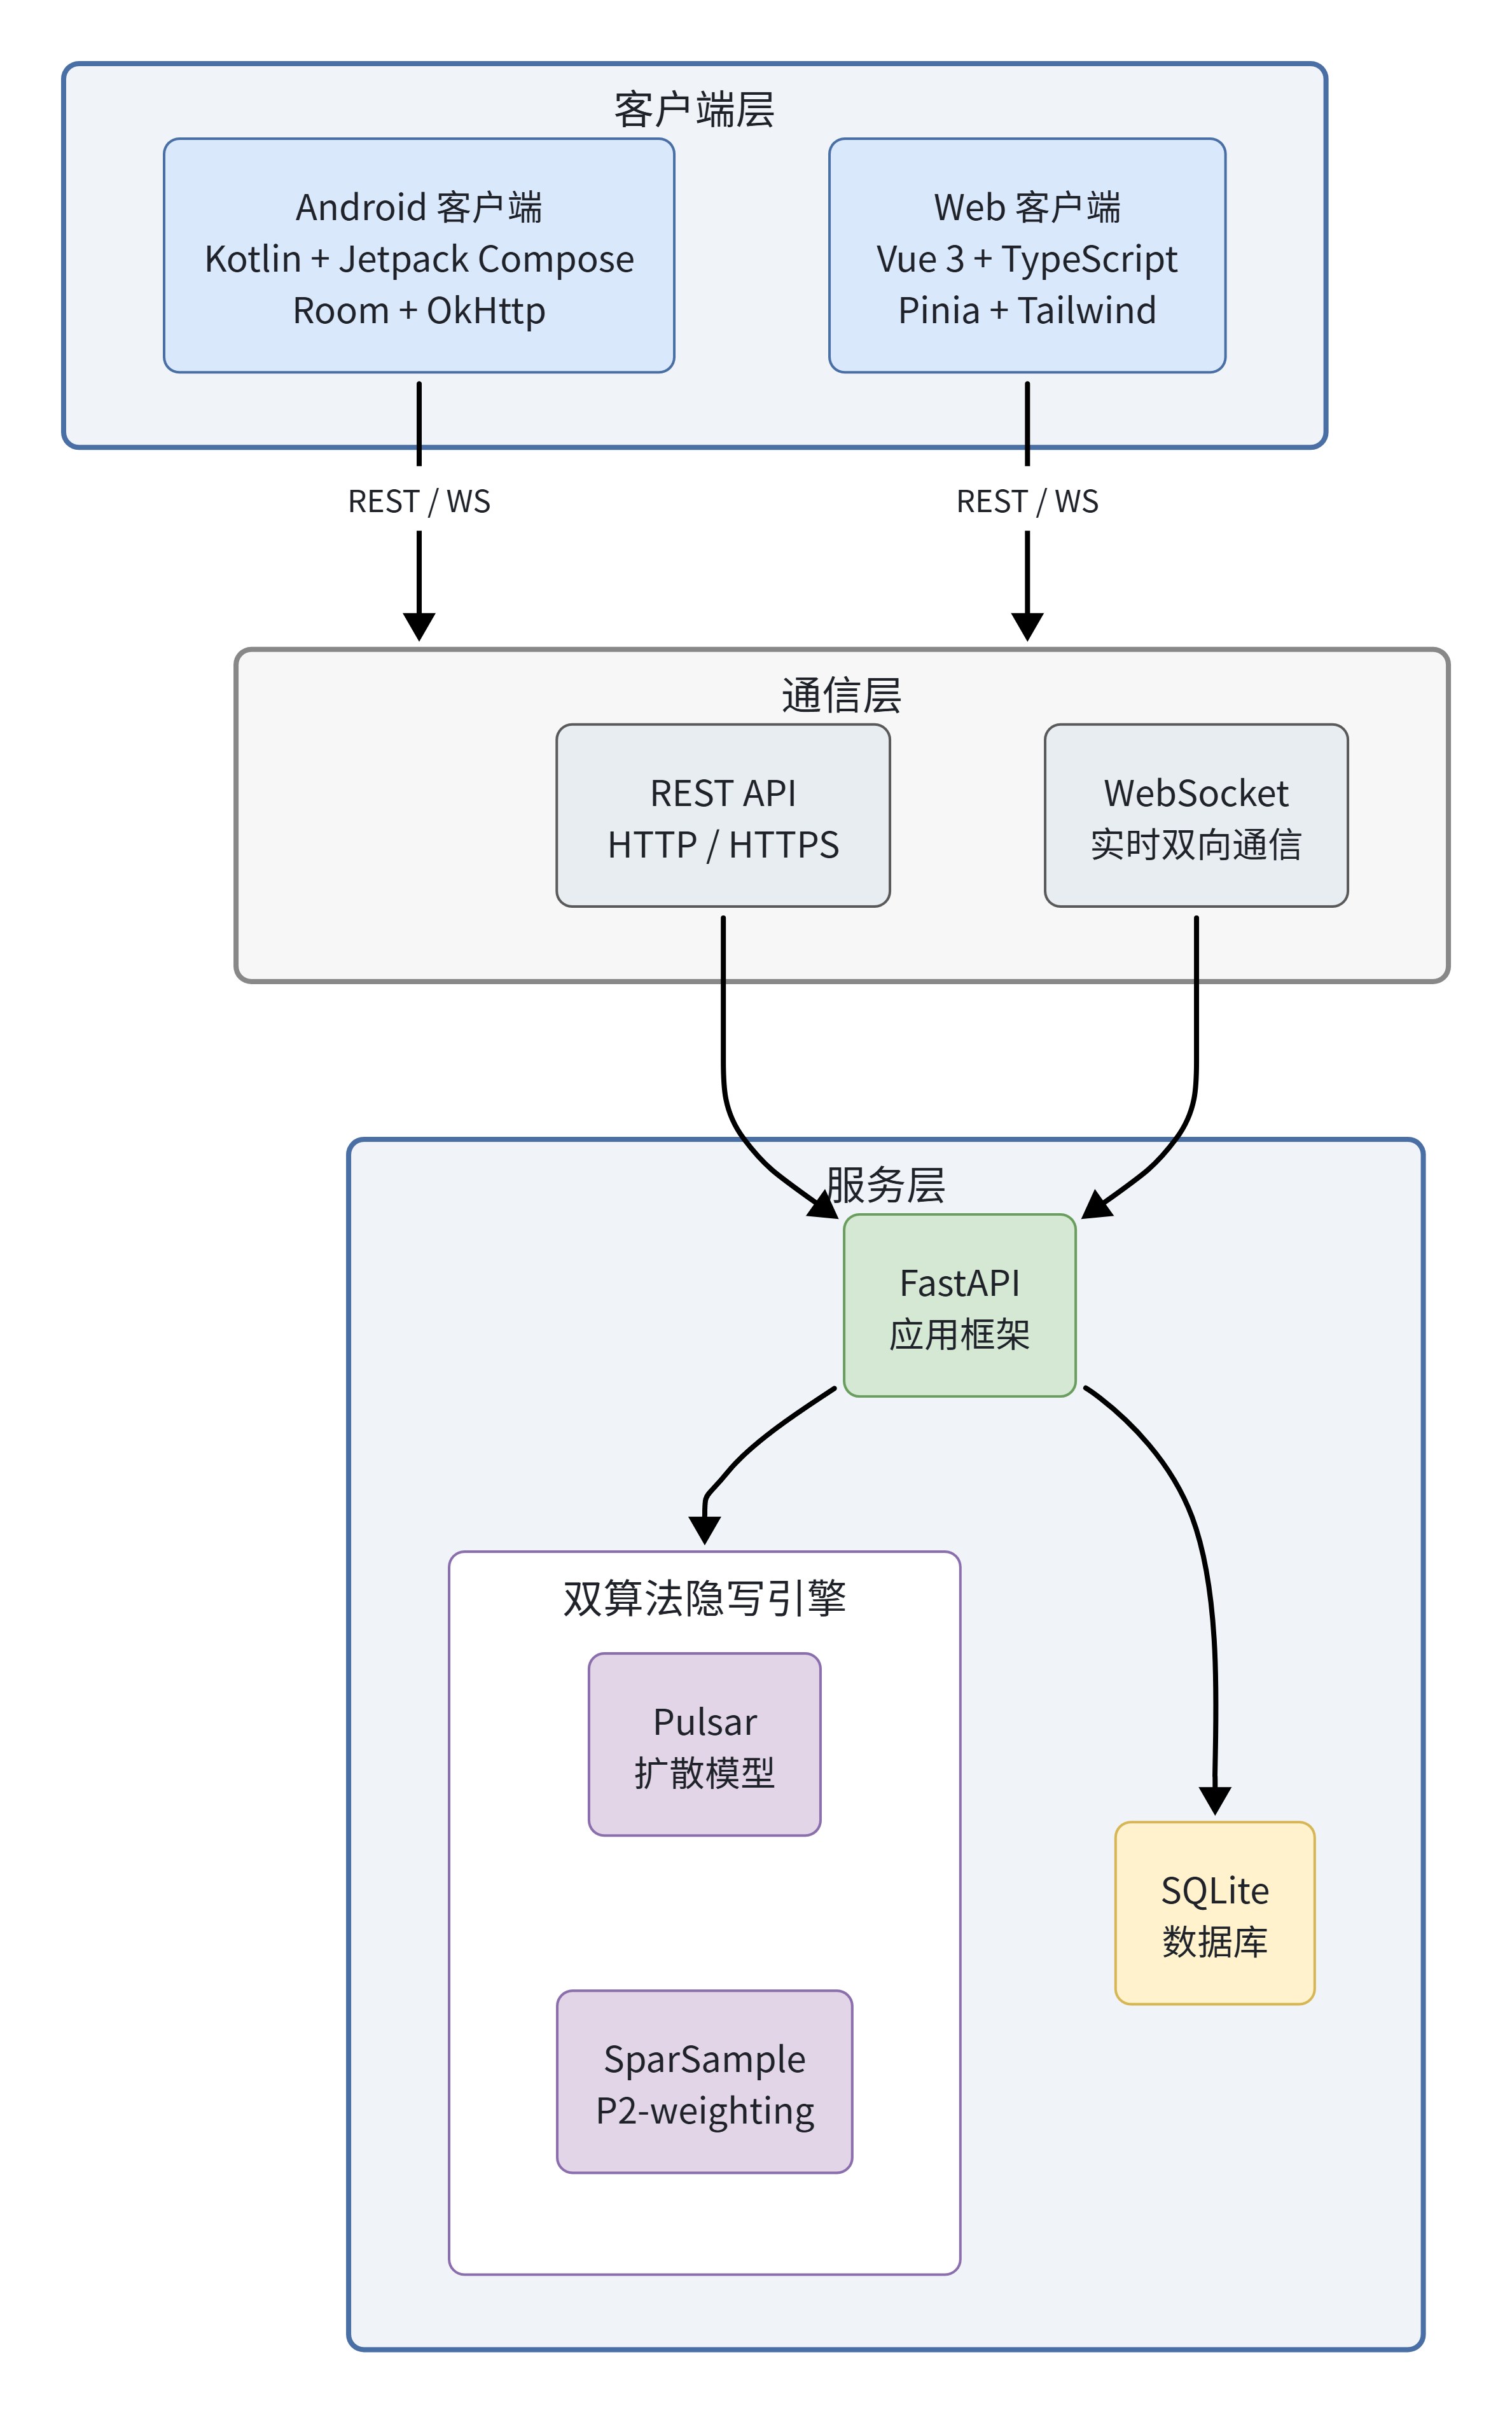
\includegraphics[width=0.85\textwidth]{img/ch3_system_arch.png}
    \caption{系统总体架构}
    \label{fig:architecture}
\end{figure}

各组件的职责分工如下：

\begin{itemize}
    \item \textbf{服务端}：负责用户认证与管理、好友关系维护、WebSocket 连接管理与消息路由、离线消息缓存、双算法隐写服务的执行（嵌入与提取计算）。服务端不接触消息明文——端到端加密在客户端完成。
    \item \textbf{Android 客户端}：提供移动端的用户界面，包括登录注册、联系人管理、聊天界面和隐写工具，使用 Room 数据库本地存储聊天记录，使用 DataStore 存储认证令牌。负责端到端加密的密钥管理和消息加解密。
    \item \textbf{Web 客户端}：提供浏览器端的用户界面，功能与 Android 客户端对齐，使用 IndexedDB 本地存储聊天记录。使用 Web Crypto API 实现密码学操作。
\end{itemize}

服务端与客户端之间通过两种通信方式交互：

\begin{itemize}
    \item \textbf{RESTful API（HTTP）}：用于用户注册登录、隐写嵌入提取、邀请码查询、算法列表查询等请求-响应式操作。
    \item \textbf{WebSocket}：用于实时消息推送、消息状态回执（已发送/已送达/已读）、消息撤回通知、好友请求通知等需要双向实时通信的场景。
\end{itemize}

\subsection{服务端设计}

\subsubsection{API 接口设计}

服务端 API 按照功能模块划分为四组路由，如\cref{tab:api}所示。

\begin{table}[htb!]
    \caption{服务端 API 接口设计}
    \centering
    \begin{tabular}{llp{5cm}}
        \hline
        \textbf{端点} & \textbf{方法} & \textbf{功能} \\
        \hline
        /api/v1/auth/register & POST & 用户注册 \\
        /api/v1/auth/login & POST & 用户登录 \\
        /api/v1/auth/me & GET & 获取当前用户信息 \\
        /api/v1/auth/logout & POST & 用户登出 \\
        /api/v1/auth/user/\{id\}/public & GET & 获取用户公开信息 \\
        \hline
        /api/v1/invite/my-code & GET & 获取自身邀请码 \\
        /api/v1/invite/reset & POST & 重置邀请码 \\
        /api/v1/invite/\{code\} & GET & 根据邀请码查找用户 \\
        /api/v1/invite/user-code/\{user\_id\} & GET & 获取指定用户邀请码 \\
        \hline
        /api/v1/stego/algorithms & GET & 获取可用算法及模型列表 \\
        /api/v1/stego/models & GET & 获取指定算法的模型列表 \\
        /api/v1/stego/embed & POST & 消息嵌入 \\
        /api/v1/stego/extract & POST & 消息提取 \\
        /api/v1/stego/capacity & POST & 容量检查 \\
        /api/v1/stego/max-capacity & GET & 获取最大容量 \\
        \hline
        /ws?token=\{jwt\} & WebSocket & 实时通信连接 \\
        \hline
    \end{tabular}
    \label{tab:api}
\end{table}

隐写相关的 API 接口均支持 \texttt{algorithm} 和 \texttt{model} 可选参数，用于指定使用哪种隐写算法和预训练模型。不指定时使用默认算法（SparSamp）和默认模型。

\subsubsection{数据库设计}

服务端使用 SQLite 数据库存储用户数据。数据库包含三张核心表，如\cref{tab:db}所示。SQLite 启用 WAL（Write-Ahead Logging）模式以提升并发读写性能。

\begin{table}[htb!]
    \caption{服务端数据库表结构}
    \centering
    \begin{tabular}{llll}
        \hline
        \textbf{表名} & \textbf{字段} & \textbf{类型} & \textbf{说明} \\
        \hline
        users & id & TEXT (PK) & 用户 UUID \\
        & username & TEXT (UNIQUE) & 用户名（3-32字符） \\
        & password\_hash & TEXT & 密码哈希（PBKDF2） \\
        & created\_at & DATETIME & 创建时间 \\
        \hline
        invite\_codes & code & TEXT (PK) & 邀请码（8位字母数字） \\
        & user\_id & TEXT (FK, UNIQUE) & 所属用户 \\
        & created\_at & DATETIME & 创建时间 \\
        \hline
        message\_queue & id & TEXT (PK) & 消息 UUID \\
        & to\_user\_id & TEXT (FK) & 目标用户 \\
        & payload & TEXT & 消息 JSON 内容 \\
        & created\_at & DATETIME & 创建时间 \\
        & expires\_at & DATETIME & 过期时间（默认24小时） \\
        \hline
    \end{tabular}
    \label{tab:db}
\end{table}

\texttt{message\_queue} 表在 \texttt{expires\_at} 和 \texttt{to\_user\_id} 字段上建立索引，以优化过期清理和用户消息查询的性能。

好友关系不存储在服务端数据库中，而是通过客户端本地数据库维护，服务端仅负责转发好友请求消息。这种设计减轻了服务端的存储负担，同时保护了用户的社交关系隐私。

\subsubsection{WebSocket 通信协议设计}

WebSocket 连接建立后，客户端和服务端通过 JSON 格式的消息进行通信。消息类型设计如\cref{tab:ws_msg}所示。

\begin{table}[htb!]
    \caption{WebSocket 消息类型}
    \centering
    \begin{tabular}{lp{7cm}}
        \hline
        \textbf{消息类型} & \textbf{说明} \\
        \hline
        chat & 普通文本聊天消息（含加密后的 SealedMessage） \\
        ack & 服务端确认收到消息，返回消息 ID 和时间戳 \\
        delivered & 消息已送达目标设备的回执 \\
        read & 消息已被目标用户阅读的回执 \\
        revoke & 消息撤回通知 \\
        typing & 正在输入指示（不持久化） \\
        friend\_request & 好友请求 \\
        friend\_accept & 接受好友请求 \\
        friend\_reject & 拒绝好友请求 \\
        first\_contact & 首次联系通知（自动触发） \\
        kicked & 单端登录踢出通知 \\
        auth\_failed & 认证失败通知 \\
        \hline
    \end{tabular}
    \label{tab:ws_msg}
\end{table}

典型的 WebSocket 通信交互流程如\cref{fig:ws_sequence}所示。

\begin{figure}[htb!]
    \centering
    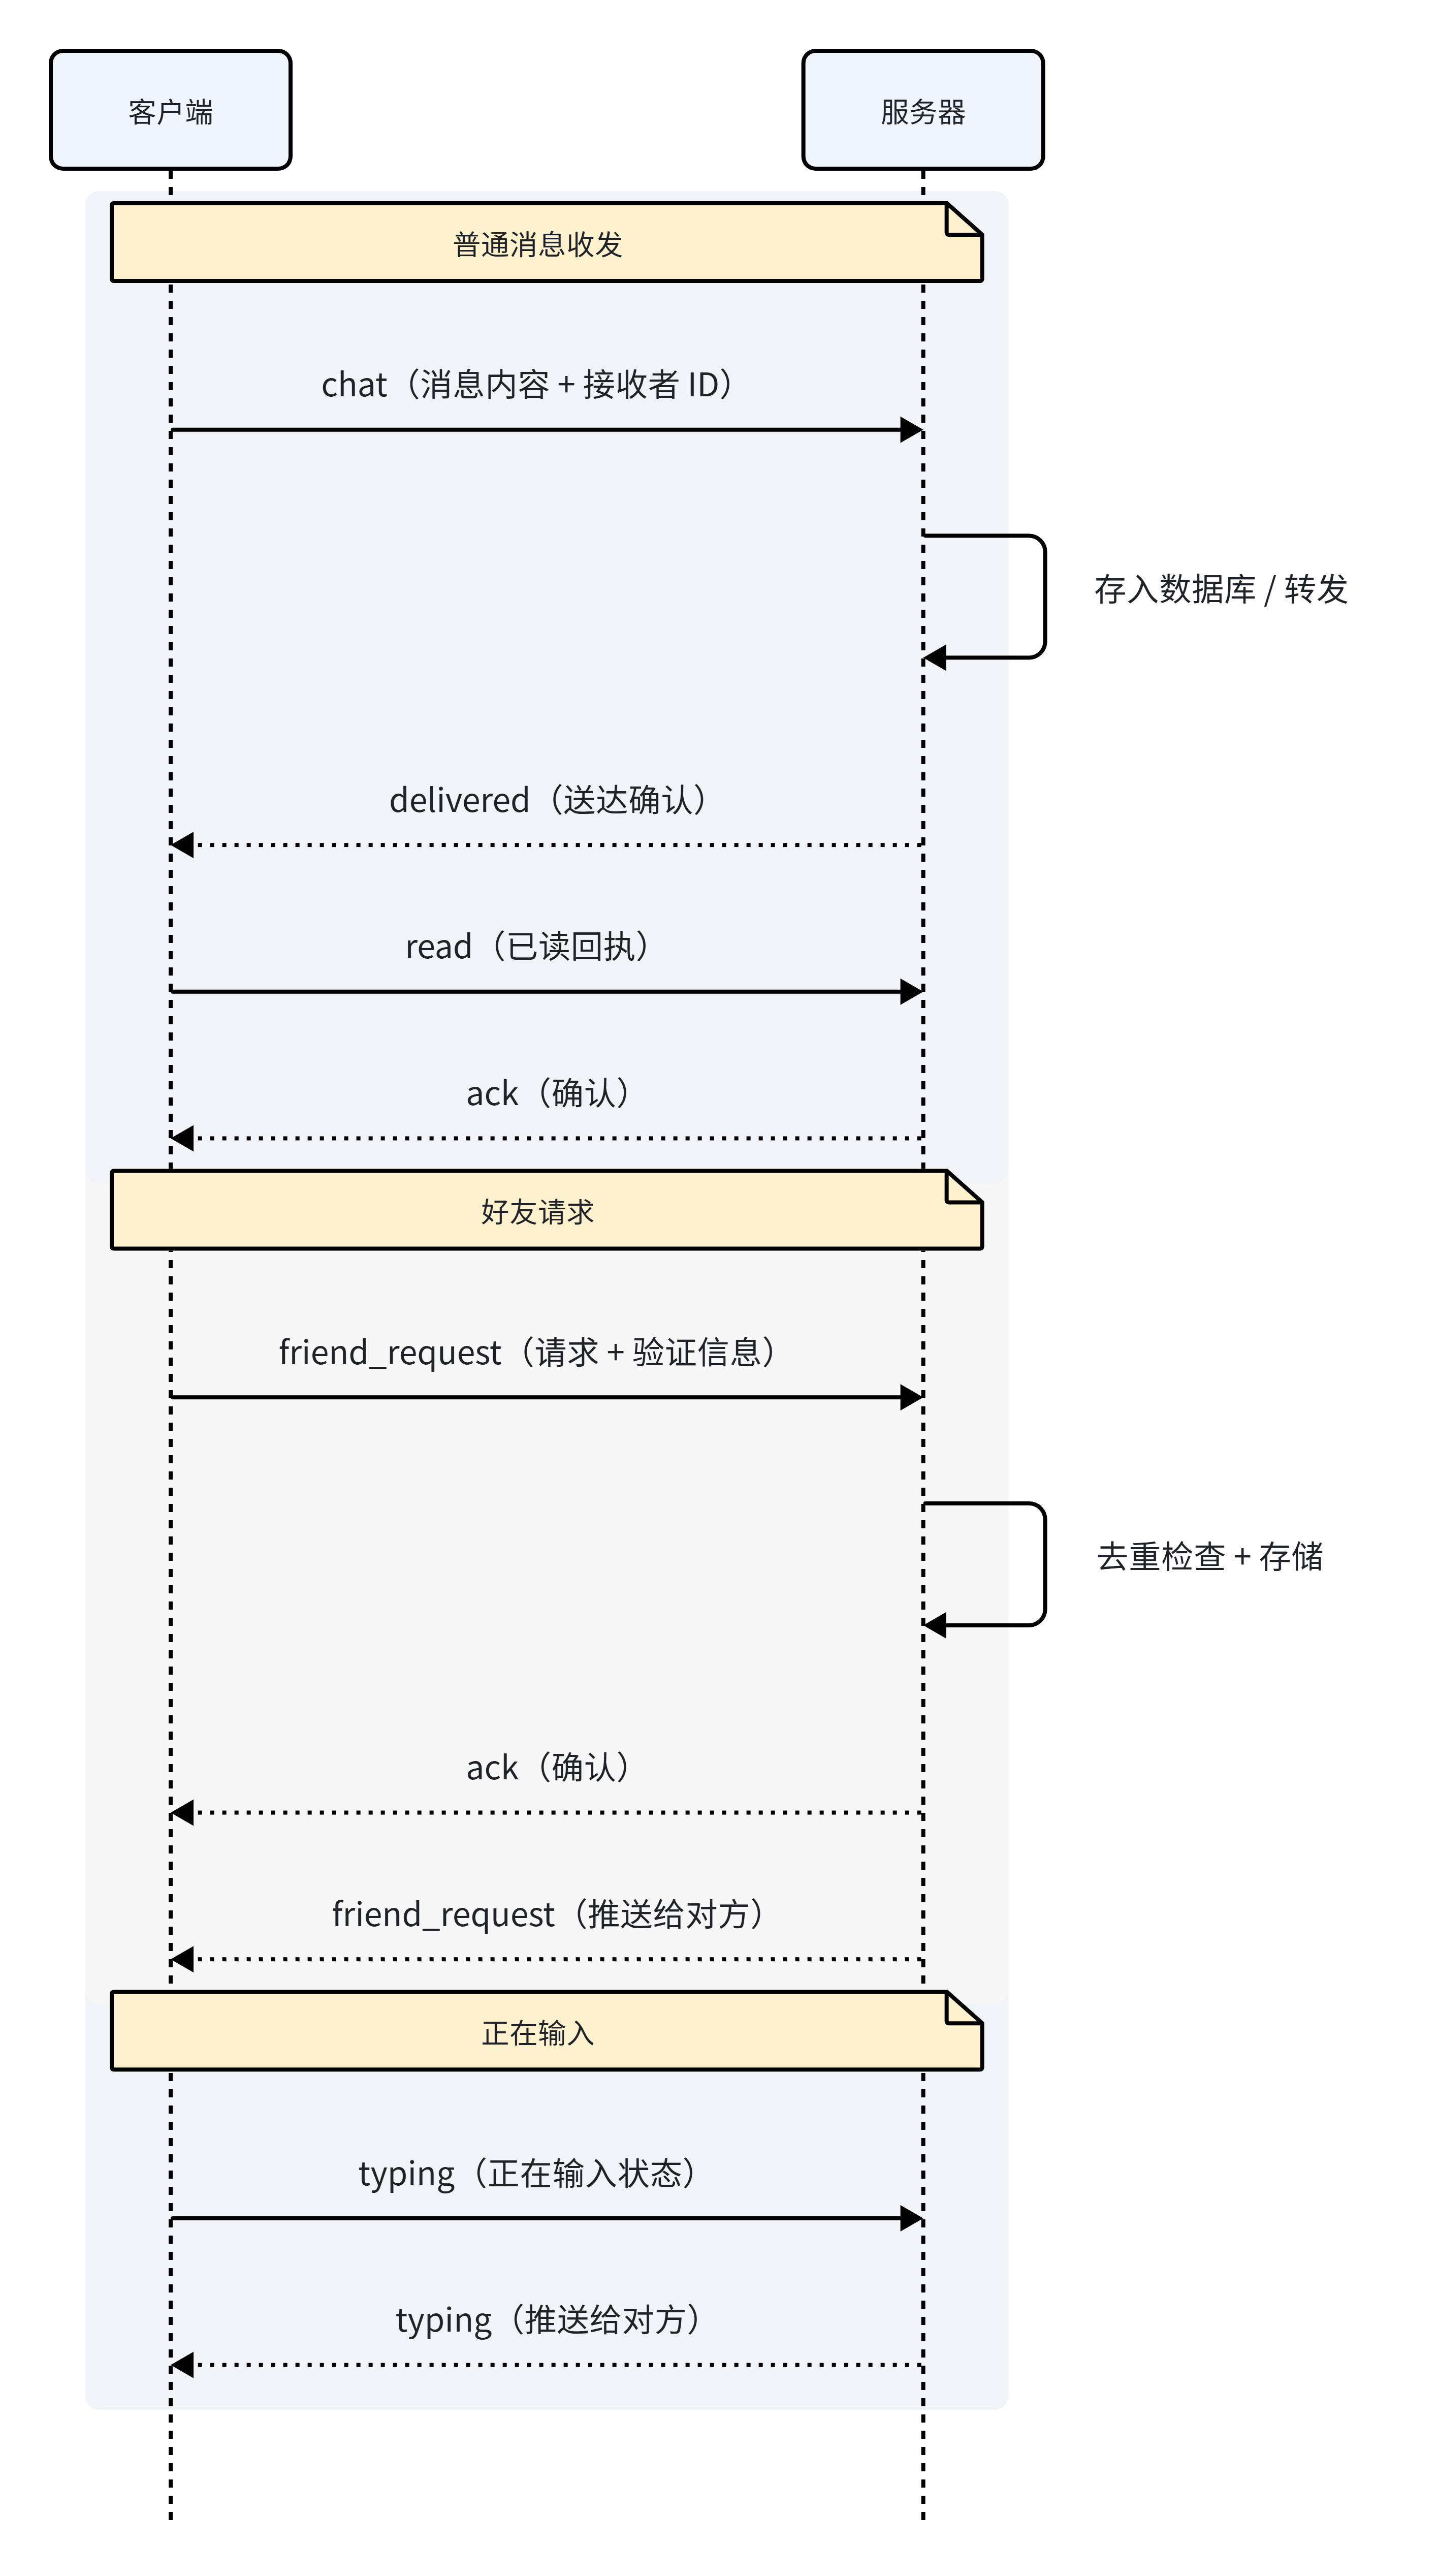
\includegraphics[width=0.85\textwidth]{img/ch3_ws_sequence.png}
    \caption{WebSocket 通信时序}
    \label{fig:ws_sequence}
\end{figure}

chat 类型的消息携带以下字段：\texttt{from\_user\_id}（发送者 ID，服务端自动填充）、\texttt{from\_username}（发送者用户名，服务端自动填充）、\texttt{to\_user\_id}（接收者 ID）、\texttt{content}（消息内容，为加密后的 SealedMessage 字符串）、\texttt{content\_type}（消息类型：text 或 stego）、\texttt{stego\_image}（隐写图像的 base64 数据，仅 stego 类型）。

\subsubsection{消息生命周期设计}

系统实现了完整的消息生命周期管理，每条消息经历以下状态变迁：

\begin{enumerate}
    \item \textbf{sending}：消息已创建，等待服务端确认。
    \item \textbf{sent}：服务端返回 ack，确认已接收消息。
    \item \textbf{delivered}：目标设备收到消息，返回 delivered 回执。
    \item \textbf{read}：目标用户阅读消息，返回 read 回执。
    \item \textbf{failed}：消息发送失败（连接断开等）。
\end{enumerate}

此外，已发送的消息支持撤回操作（revoke），撤回后消息内容被清除，显示"消息已撤回"状态。撤回操作有时间限制（默认 120 秒）。消息状态变迁如\cref{fig:msg_state}所示。

\begin{figure}[htb!]
    \centering
    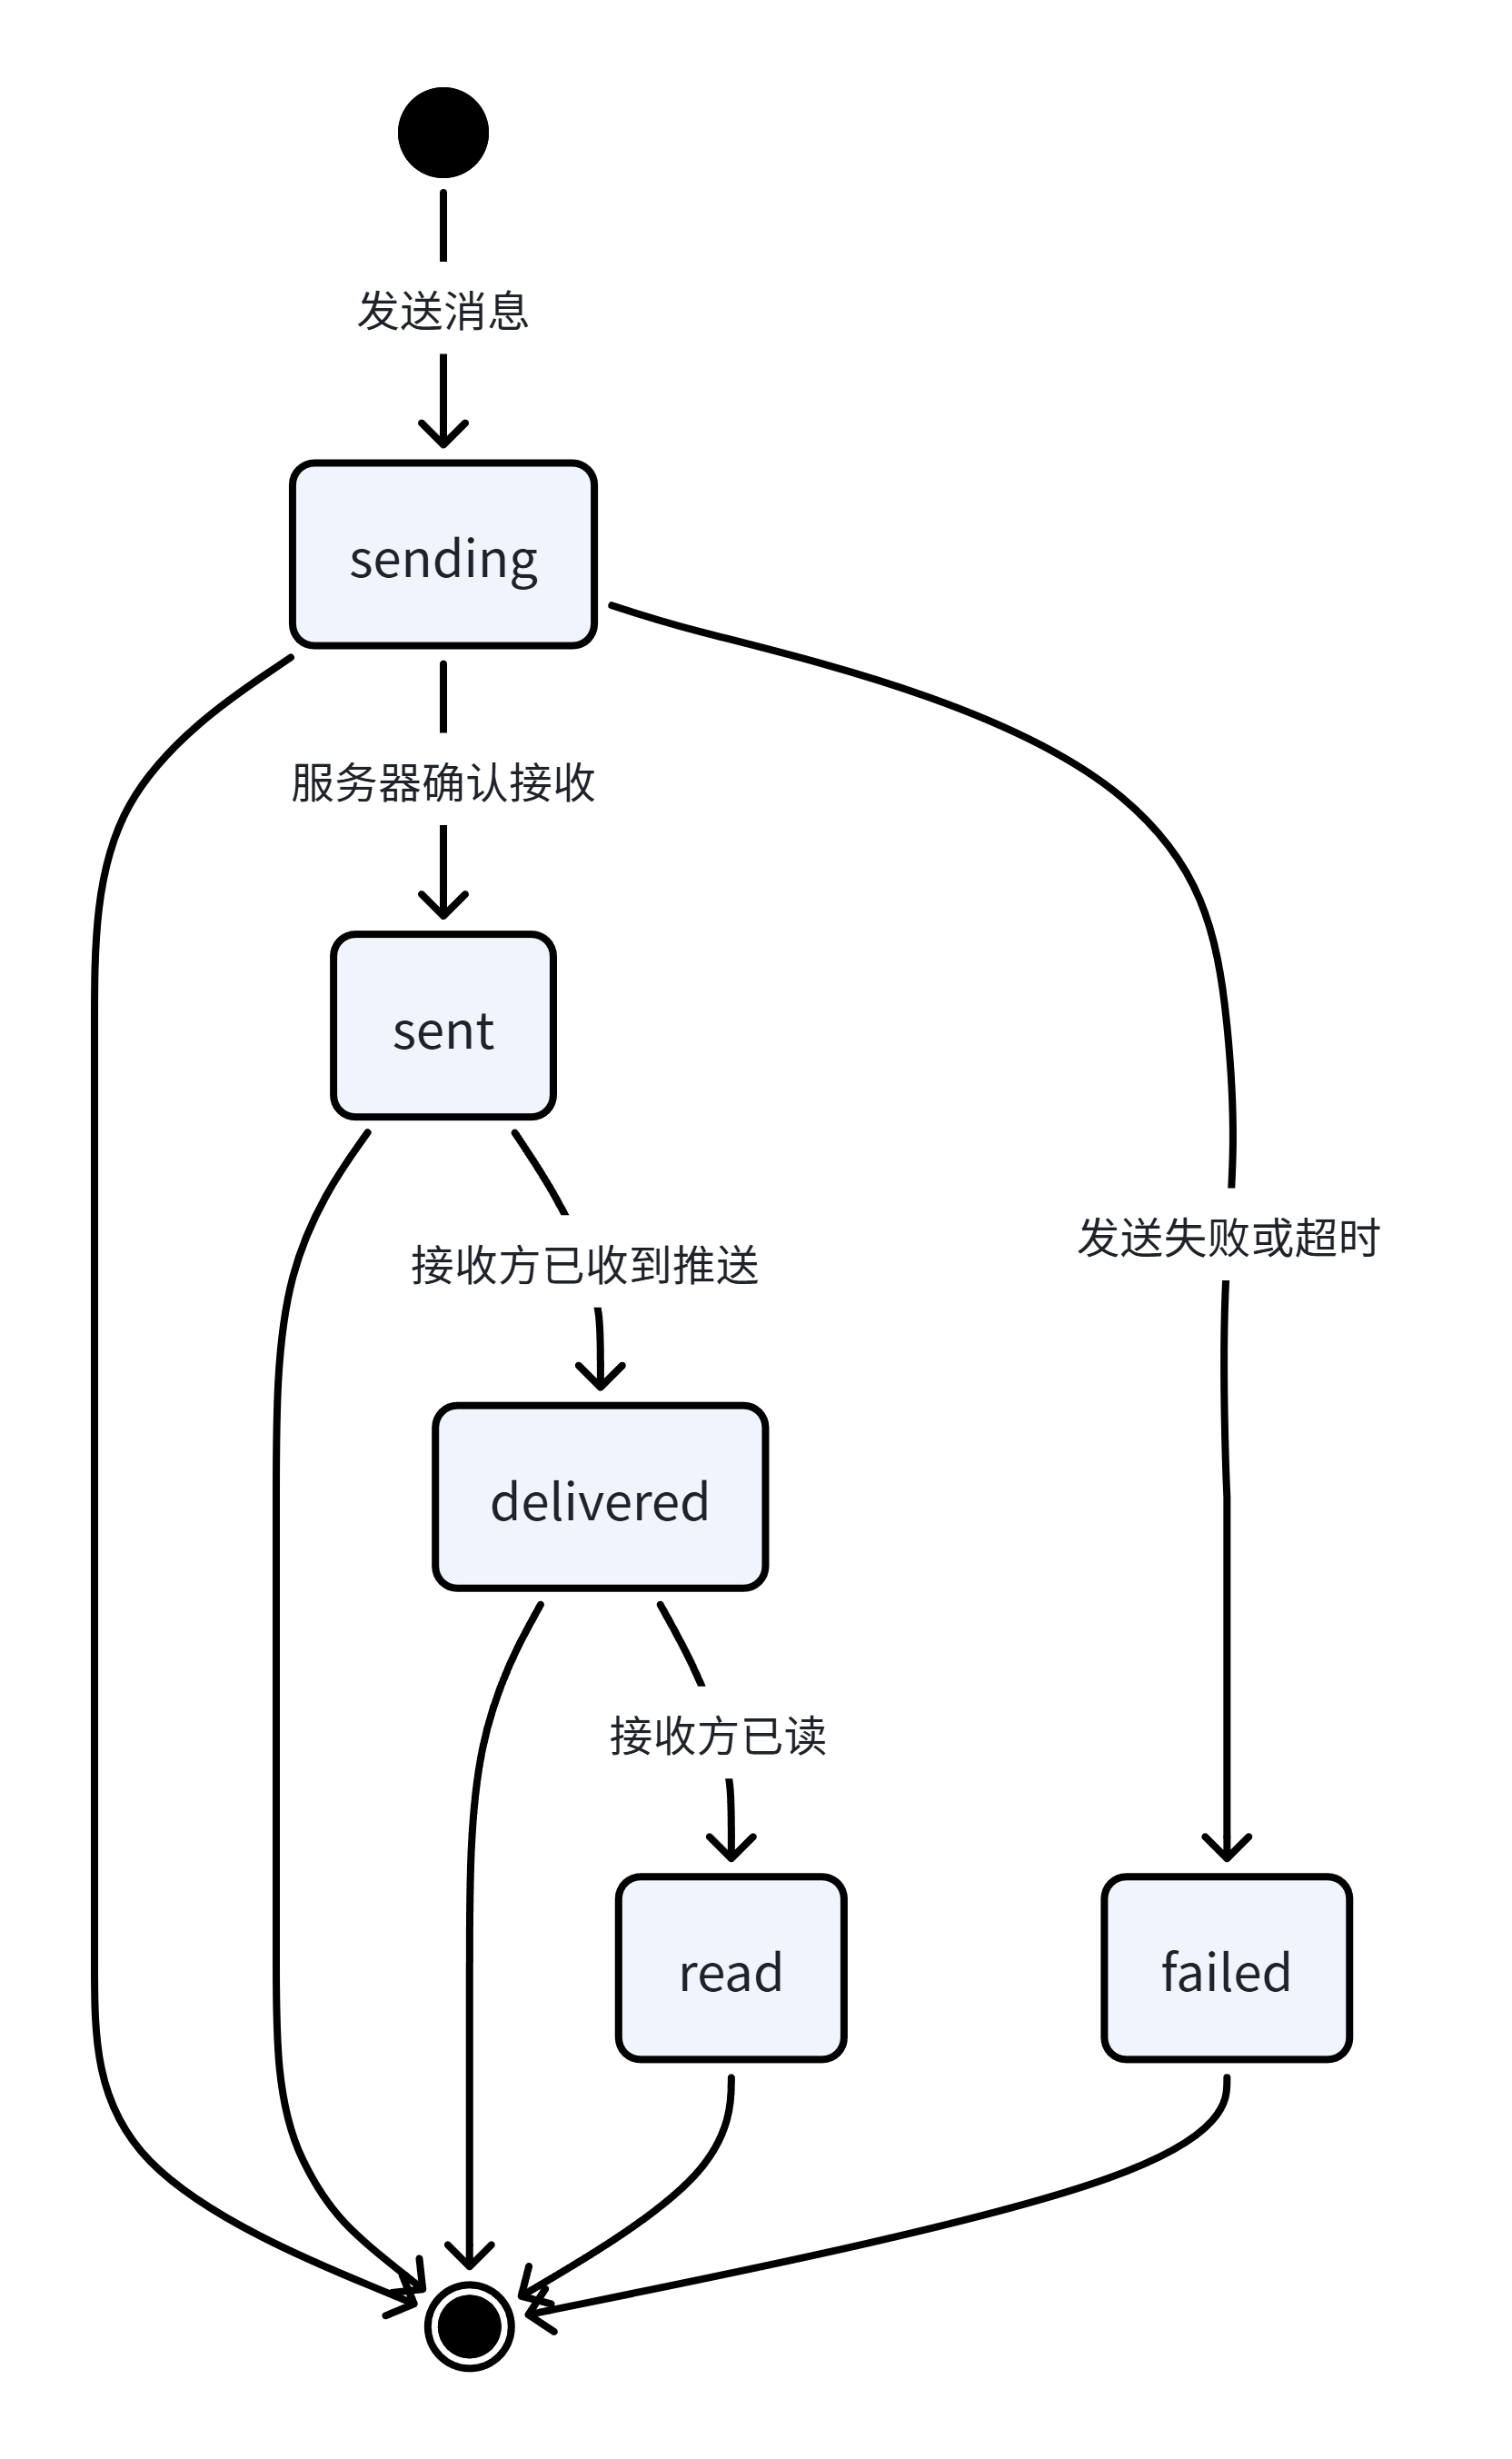
\includegraphics[width=0.6\textwidth]{img/ch3_msg_state.png}
    \caption{消息状态机}
    \label{fig:msg_state}
\end{figure}

\subsubsection{离线消息队列设计}

当目标用户不在线时，服务端将消息暂存于 \texttt{message\_queue} 表中，并设置过期时间（默认 24 小时）。当用户重新连接 WebSocket 时，服务端自动查询并投递该用户的所有未过期离线消息，投递完成后从队列中删除。同时，服务端启动定时任务每 5 分钟清理过期消息。

\subsubsection{双算法隐写服务设计}

隐写服务采用统一的算法注册表模式，支持 Pulsar 和 SparSamp 两种算法并行运行。算法注册表维护每个算法的元信息（名称、模型列表、服务类），以及默认算法标识。

\begin{itemize}
    \item \textbf{Pulsar 服务}：封装外部 Pulsar Python 包，支持 CelebA-HQ、Church、Bedroom、Cat 四种预训练 DDPM 模型。模型文件通过 HuggingFace Hub 或本地目录加载。
    \item \textbf{SparSamp 服务}：基于项目内实现的 IDDPM P2-weighting 框架，支持 FFHQ、AFHQ Dog、Flower、CUB 四种预训练模型。模型文件为 \texttt{.pt} 格式，存放在 \texttt{models/sparsample/} 目录下。
\end{itemize}

两种算法均通过 \texttt{run\_in\_threadpool} 在线程池中执行，避免阻塞异步事件循环。每个（算法、模型、密钥）组合对应一个独立的算法实例，通过字典缓存实现复用。

\subsection{客户端设计}

\subsubsection{Android 客户端架构}

Android 客户端采用 MVVM（Model-View-ViewModel）架构模式，如\cref{fig:android_arch}所示。

\begin{figure}[htb!]
    \centering
    \begin{tabular}{|c|}
        \hline
        \textbf{View 层}：Jetpack Compose UI 组件 \\
        AuthScreen / ChatListScreen / ChatScreen / ContactsScreen \\
        AddContactScreen / ContactDetailScreen / RequestsScreen \\
        ProfileScreen / StegoToolScreen \\
        \hline
    \end{tabular}

    \vspace{0.3cm}
    $\Updownarrow$
    \vspace{0.3cm}

    \begin{tabular}{|c|}
        \hline
        \textbf{ViewModel 层}：状态管理与业务逻辑 \\
        AuthViewModel / ChatViewModel / ContactViewModel / ProfileViewModel \\
        \hline
    \end{tabular}

    \vspace{0.3cm}
    $\Updownarrow$
    \vspace{0.3cm}

    \begin{tabular}{|c|}
        \hline
        \textbf{Model 层}：数据访问 \\
        Room 数据库 / Retrofit 网络 / OkHttp WebSocket / DataStore / CryptoUtils \\
        \hline
    \end{tabular}
    \caption{Android 客户端 MVVM 架构}
    \label{fig:android_arch}
\end{figure}

Android 客户端包含 36 个 Kotlin 源文件，按功能划分为以下包：

\begin{itemize}
    \item \textbf{api/}：API 客户端（Retrofit 接口定义和 DTO 数据类）。
    \item \textbf{crypto/}：端到端加密工具类（密钥派生、AES-GCM 加解密、SealedMessage 信封）。
    \item \textbf{data/local/}：本地数据存储（Room 数据库、DataStore、DAO）。
    \item \textbf{data/remote/}：WebSocket 客户端。
    \item \textbf{ui/navigation/}：导航图定义。
    \item \textbf{ui/screens/}：各页面的 Composable 函数。
    \item \textbf{ui/theme/}：Material 3 主题定义（颜色、字体、形状）。
    \item \textbf{ui/viewmodel/}：ViewModel 层。
\end{itemize}

底部导航栏提供四个入口：消息（会话列表）、联系人、隐写工具和我的（个人设置）。

\subsubsection{Web 客户端架构}

Web 客户端采用 Vue.js 3 组合式 API 开发，使用 Pinia 进行集中式状态管理。

\begin{itemize}
    \item \textbf{视图层}：Vue 单文件组件（SFC），共 10 个页面组件和 3 个公共组件。
    \item \textbf{状态管理层}：Pinia Store 管理全局状态，包括 AuthStore（认证状态）、ChatStore（聊天与 WebSocket 连接、E2EE 消息密钥管理）、ContactStore（联系人管理）、SettingsStore（自身 E2EE 配置）。
    \item \textbf{数据持久层}：使用 IndexedDB（通过 idb 库封装）存储聊天消息、联系人数据、黑名单和 E2EE 配置。
    \item \textbf{API 层}：使用 Axios 发送 HTTP 请求，自动注入 JWT 令牌。
    \item \textbf{WebSocket 层}：使用浏览器原生 WebSocket API，封装为 WsClient 类，支持指数退避重连。
    \item \textbf{密码学层}：使用 Web Crypto API 实现 E2EE 密钥派生和消息加解密。
\end{itemize}

Web 客户端采用 Aegis Slate 暗色 Material 3 设计系统，主色调为深海军蓝（\#0b1326），强调色为蓝色（\#adc6ff），使用 Tailwind CSS 实现响应式布局。侧边导航栏宽 64px，提供会话、联系人、工具和设置四个导航入口。Web 客户端架构如\cref{fig:web_arch}所示。

\begin{figure}[htb!]
    \centering
    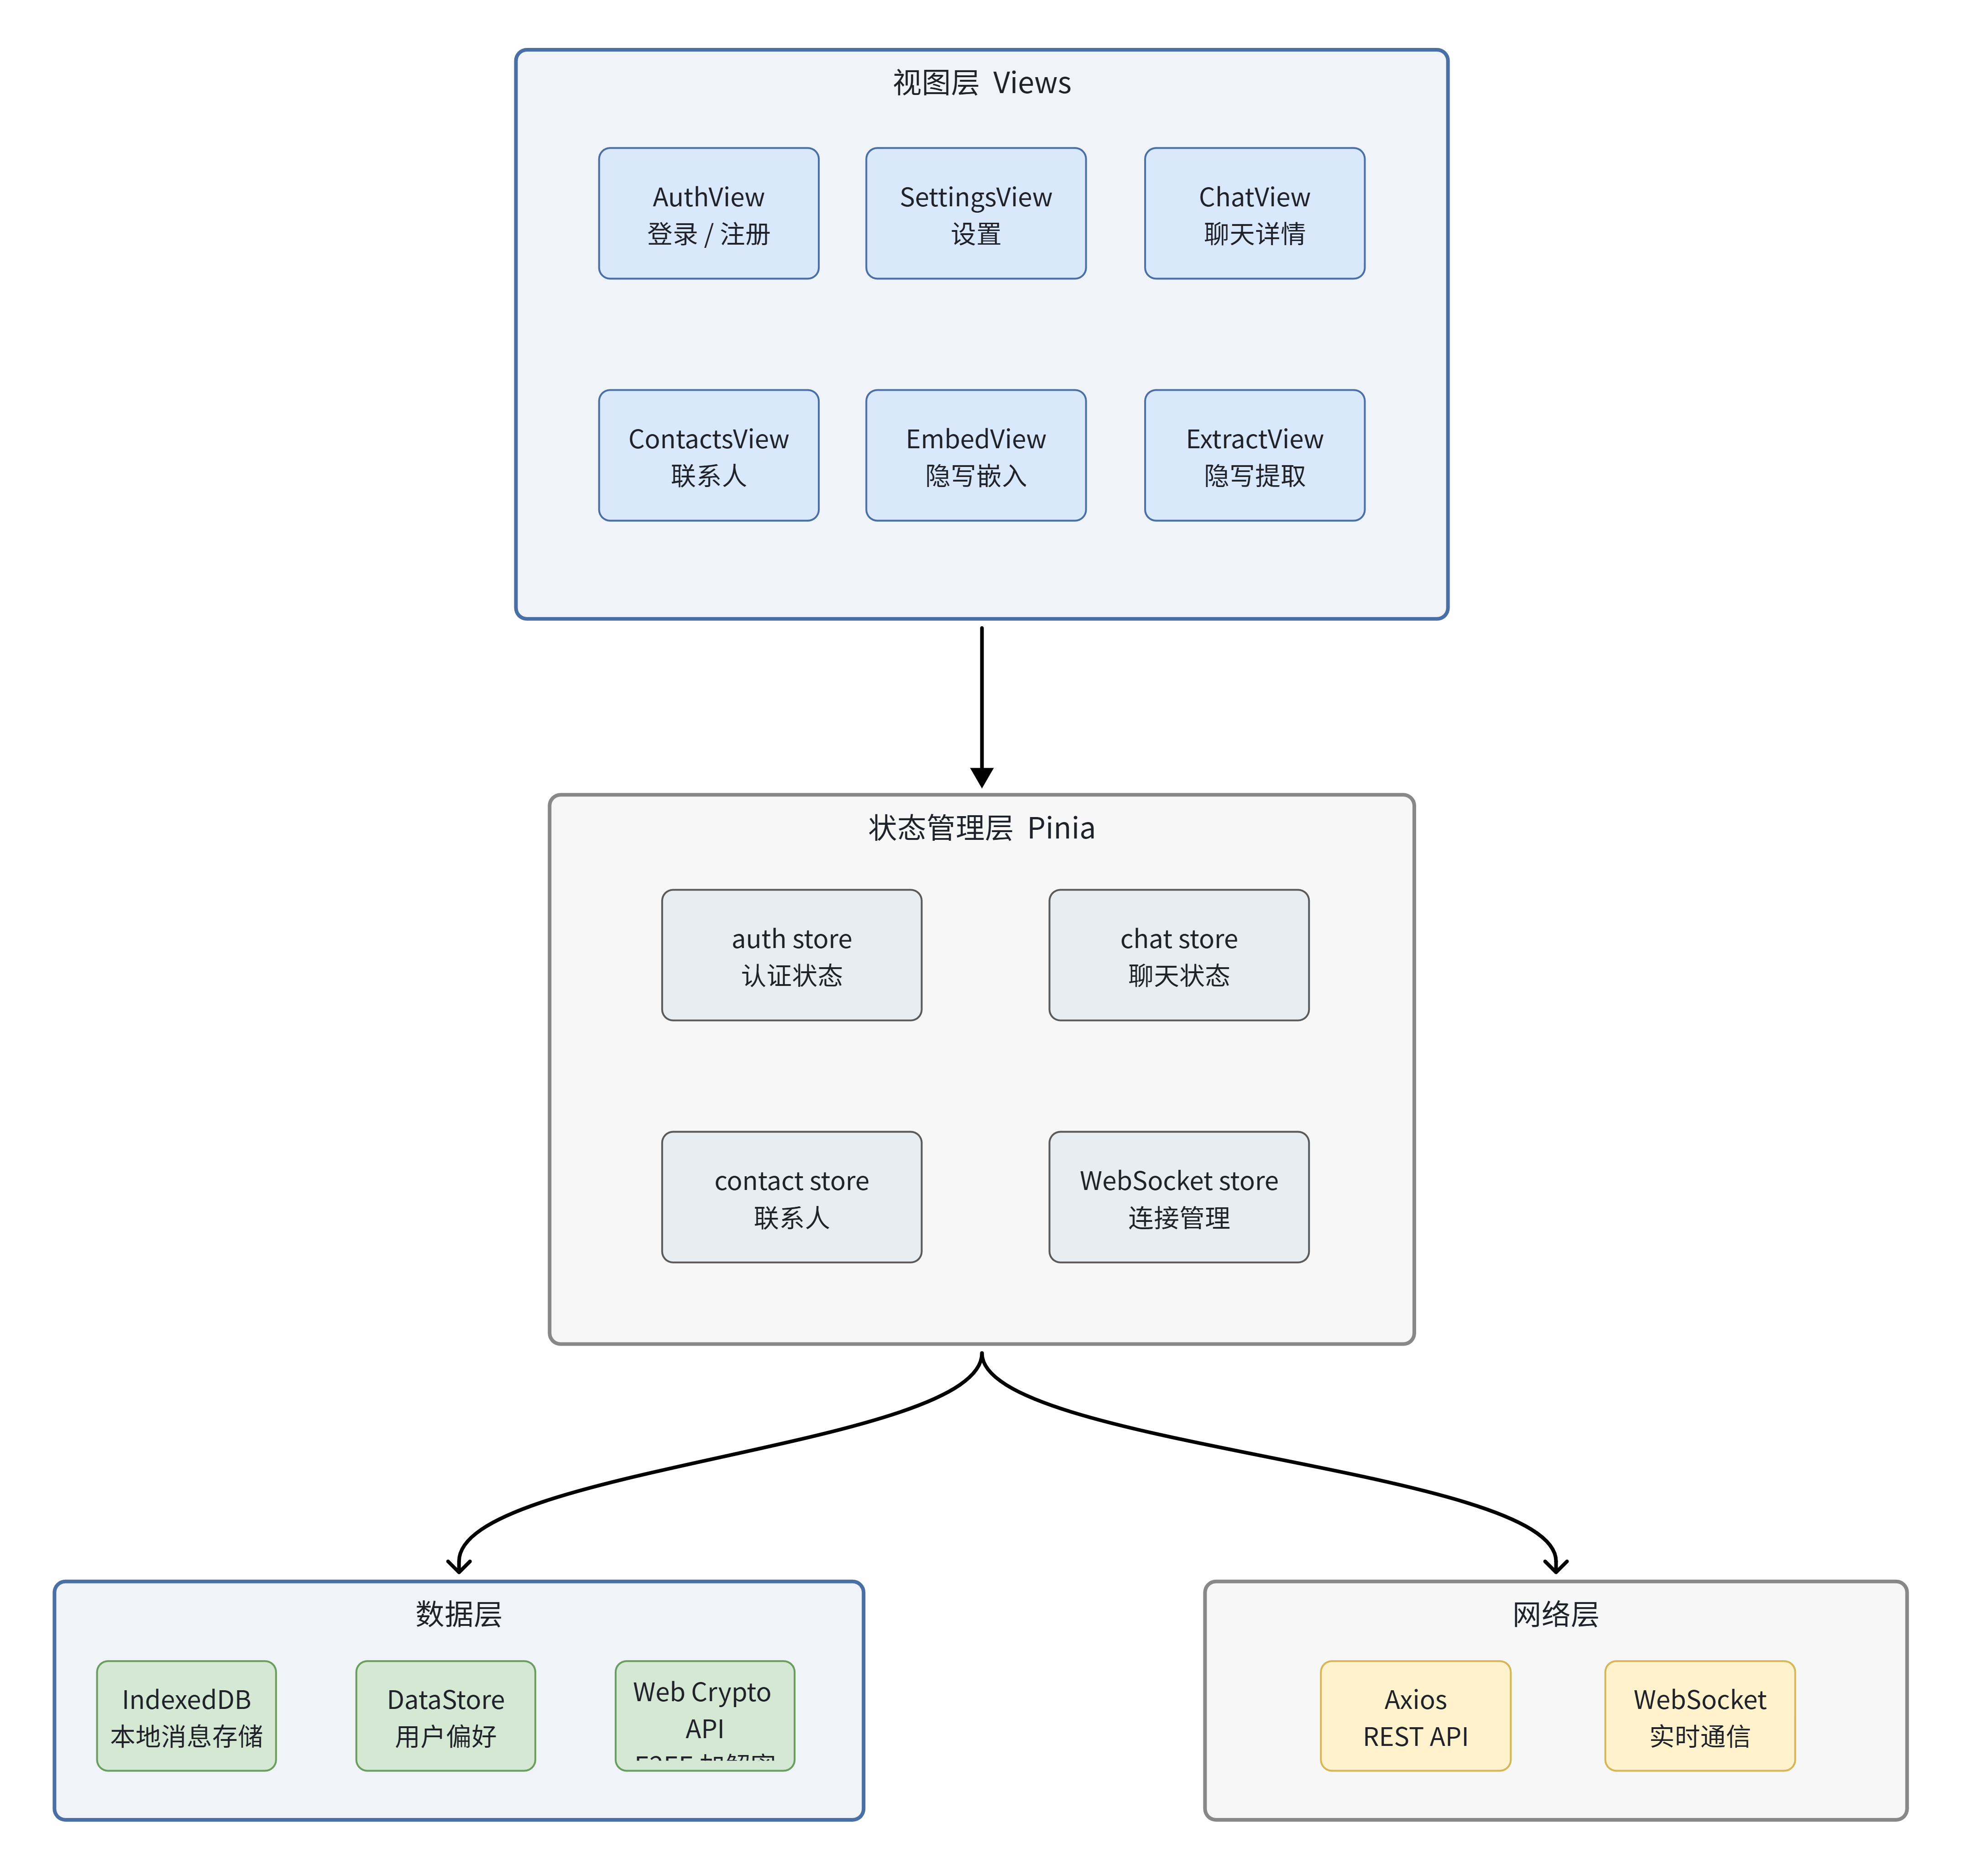
\includegraphics[width=0.85\textwidth]{img/ch3_web_arch.png}
    \caption{Web 客户端架构}
    \label{fig:web_arch}
\end{figure}

\subsubsection{本地存储设计}

Android 客户端的 Room 数据库（版本 2）包含以下实体：

\begin{itemize}
    \item \textbf{ContactEntity}：联系人信息（用户ID、用户名、状态、添加时间、对方助记词、对方用户密钥十六进制、对方指纹十六进制）。
    \item \textbf{MessageEntity}：聊天消息（消息ID、联系人ID、方向、内容、内容类型、隐写图像、状态、撤回标记、创建时间）。
    \item \textbf{BlacklistEntity}：黑名单（用户ID、用户名、屏蔽时间）。
    \item \textbf{UserSettingsEntity}：当前用户的 E2EE 配置（助记词、用户密钥十六进制、指纹十六进制），单行表。
\end{itemize}

Web 客户端的 IndexedDB 数据库（数据库名 \texttt{stego-app}，版本 2）包含四个对象存储：\texttt{contacts}、\texttt{messages}、\texttt{blacklist}、\texttt{settings}，结构与 Android 端对应。

\subsection{安全设计}

\subsubsection{威胁模型}

本系统的安全设计基于以下威胁模型和信任假设：

\begin{itemize}
    \item \textbf{攻击者能力}：假设攻击者能够被动监听服务端的所有通信流量，包括 WebSocket 消息和 HTTP 请求；能够获取服务端数据库的完整内容（含用户密码哈希、邀请码和离线消息队列）；能够截获并读取客户端与服务端之间的所有网络数据包。
    \item \textbf{安全目标}：即使攻击者具备上述能力，也无法获取用户聊天消息的明文内容（消息机密性）；无法伪造合法用户的消息（消息完整性与认证性）；无法确定含密图像中是否隐藏了秘密信息（隐写不可检测性）。
    \item \textbf{信任假设}：用户信任自己所使用的客户端应用（Android 或 Web）未被篡改；助记词短语通过安全的带外渠道（如面对面）在通信双方之间共享；隐写算法本身的可证安全性基于底层扩散模型的 KL 散度保证。
\end{itemize}

需要注意的是，当前系统的隐写密钥通过邀请码 XOR 派生，而邀请码存储在服务端数据库中，因此隐写密钥的安全性依赖于服务端的可信度。这是系统在安全性方面的一个已知局限，详见\cref{sec:future_work}的讨论。

\subsubsection{JWT 认证机制}

系统使用 JSON Web Token（JWT）进行用户身份认证。用户登录成功后，服务端签发包含用户ID和用户名的 JWT 令牌，有效期为 7 天。客户端在后续的 HTTP 请求中通过 Authorization 头部携带令牌，WebSocket 连接通过 URL 查询参数传递令牌。服务端使用 HMAC-SHA256（HS256）算法验证令牌的完整性和有效性。

JWT 密钥通过三级降级策略生成和持久化：优先读取环境变量 \texttt{JWT\_SECRET}，其次读取项目目录下的 \texttt{.jwt\_secret} 文件，最后随机生成并写入文件（权限 0600），确保服务重启后已有令牌不会失效。

\subsubsection{密码安全}

用户密码使用 PBKDF2-HMAC-SHA256 算法进行哈希存储，迭代次数为 100,000 次，每个用户使用随机生成的 UUID4 作为盐值。迭代次数的选择基于实际部署环境的权衡：OWASP 2023 年推荐的最低迭代次数为 600,000 次，但本系统的服务端运行在普通开发硬件上，100,000 次迭代已能在保证安全强度的同时维持登录响应在 200ms 以内。对于生产环境部署，建议将迭代次数提升至 600,000 次以上。哈希结果以十六进制编码，存储格式为 \texttt{盐值\textdollar 哈希值}。验证时使用 \texttt{hmac.compare\_digest} 进行时间安全比较，防止时序攻击。

\subsubsection{端到端加密设计}

端到端加密的密钥管理遵循以下原则：

\begin{itemize}
    \item \textbf{助记词本地存储}：用户的助记词短语和派生的用户密钥仅存储在客户端本地数据库中，不传输到服务端。
    \item \textbf{消息密钥内存驻留}：对称消息密钥（mkey）仅在 ViewModel 的内存变量中存在，不进行持久化存储，每次切换聊天对象时重新计算。
    \item \textbf{密文传输}：所有聊天消息在客户端加密为 SealedMessage 格式后传输，服务端只看到密文。
    \item \textbf{指纹验证}：用户可通过对比对方的密钥指纹（8 字节 SHA-256 摘要）来验证密钥配对的正确性。
\end{itemize}

\subsubsection{隐写密钥派生}

在隐写聊天模式下，系统自动使用通信双方的邀请码进行 XOR 运算生成隐写密钥。XOR 运算具有对称性，双方无需协商即可独立计算出相同的密钥。生成的密钥以十六进制字符串形式传递给隐写 API，作为伪随机数生成器的种子。

\subsubsection{单端登录策略}

为防止多设备同时登录引发的数据一致性问题，系统实施单端登录策略。当用户在新设备登录时，服务端向旧连接发送 \texttt{kicked} 消息通知其被踢出，旧客户端收到通知后清除本地令牌并跳转到登录页面。5 秒后服务端强制关闭旧连接作为兜底措施。主动登出清除所有本地数据，而被踢出仅清除令牌，保留聊天记录便于用户重新登录后查看。

\subsection{本章小结}

本章从功能需求和非功能需求出发，设计了系统的总体架构，详细阐述了服务端的 API 接口、数据库、WebSocket 通信协议（含完整的消息生命周期）、离线消息队列和双算法隐写服务的设计方案，以及客户端的架构和本地存储设计。同时，从 JWT 认证、密码安全、端到端加密、隐写密钥派生和单端登录五个方面介绍了系统的安全设计。
